\documentclass[12pt]{article}
\usepackage[margin=2.5cm]{geometry}
\usepackage{enumerate}
\usepackage{amsfonts}
\usepackage{amsmath}
\usepackage{fancyhdr}
\usepackage{amsmath}
\usepackage{amssymb}
\usepackage{amsthm}
\usepackage{mdframed}
\usepackage{graphicx}
\usepackage{subcaption}
\usepackage{adjustbox}
\usepackage{listings}
\usepackage{xcolor}
\usepackage{booktabs}
\usepackage[utf]{kotex}
\usepackage{hyperref}

\definecolor{codegreen}{rgb}{0,0.6,0}
\definecolor{codegray}{rgb}{0.5,0.5,0.5}
\definecolor{codepurple}{rgb}{0.58,0,0.82}
\definecolor{backcolour}{rgb}{0.95,0.95,0.92}

\lstdefinestyle{mystyle}{
    backgroundcolor=\color{backcolour},
    commentstyle=\color{codegreen},
    keywordstyle=\color{magenta},
    numberstyle=\tiny\color{codegray},
    stringstyle=\color{codepurple},
    basicstyle=\ttfamily\footnotesize,
    breakatwhitespace=false,
    breaklines=true,
    captionpos=b,
    keepspaces=true,
    numbers=left,
    numbersep=5pt,
    showspaces=false,
    showstringspaces=false,
    showtabs=false,
    tabsize=1
}

\lstset{style=mystyle}

\pagestyle{fancy}
\renewcommand{\headrulewidth}{0.4pt}
\lhead{Hyungmo Gu}
\rhead{CSC369 Week 8 Notes}

\begin{document}
\title{CSC369 Week 8 Notes}
\author{Hyungmo Gu}
\maketitle

\begin{itemize}
    \item File Systems
    \begin{itemize}
        \item Is the part of operating system dealing with files $^{[2]}$
        \item Controls how data is stored and retrieved. $^{[1]}$
        \begin{itemize}
            \item Without a file system, data placed in a storage medium is one
            large body of data with no way to tell where it stops and the next begins
        \end{itemize}
    \end{itemize}

    \begin{center}
    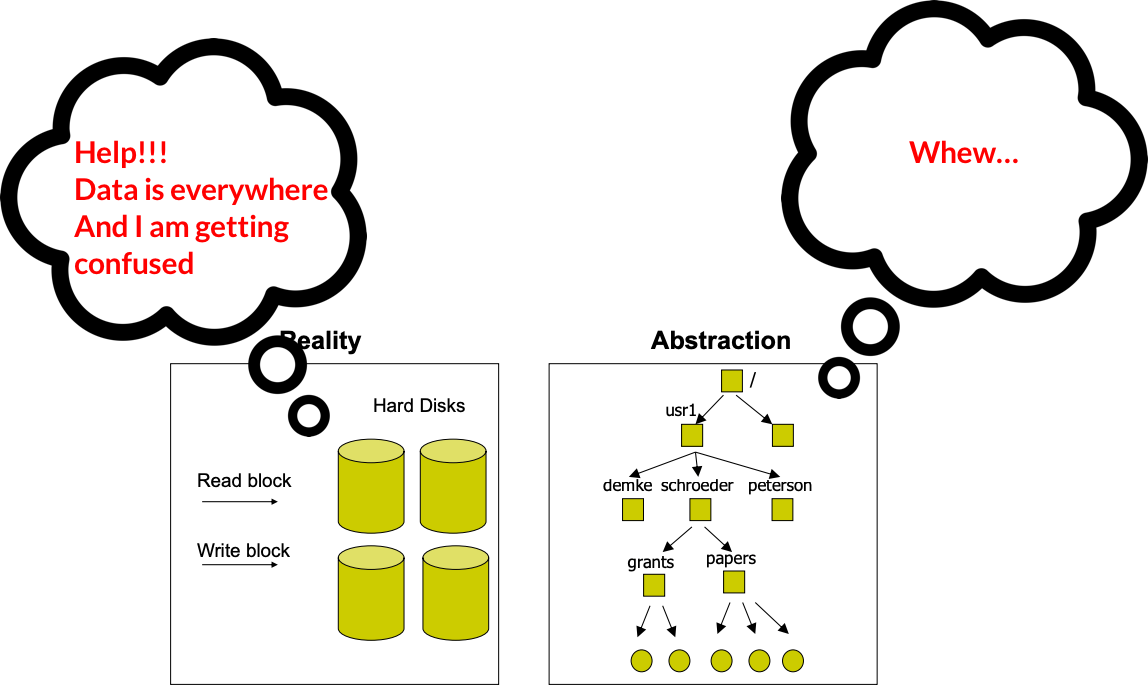
\includegraphics[width=0.8\linewidth]{images/week_8_notes_1_1.png}
    \end{center}

    \bigskip

    \underline{\textbf{Refernces:}}

    \bigskip

    \begin{enumerate}[1)]
        \item Wikipedia: File Systems, \href{https://en.wikipedia.org/wiki/Paging}{link}
        \item Tanebaum AS, Boss H. 2015. Modern Operating Systems. 4th Edition. New Jersy: Pearson Education, Inc.
    \end{enumerate}
    \item File Concept
    \begin{itemize}
        \item Files
        \begin{itemize}
            \item Are logical units of information created by processes $^{[1]}$
            \item Is named collection of data with some attributes
            \begin{enumerate}[1.]
                \item Name
                \item Owner
                \item Location
                \item Size
                \item Protection
                \item Creation Time
                \item Time of Last Access
            \end{enumerate}
        \end{itemize}

    \end{itemize}

    \bigskip

    \underline{\textbf{Refernces:}}

    \bigskip

    \begin{enumerate}[1)]
        \item Tanebaum AS, Boss H. 2015. Modern Operating Systems. 4th Edition. New Jersy: Pearson Education, Inc.
    \end{enumerate}
    % \item File Types
    % \item Conceptual File Operation
    % \item File Access Methods
    % \item Handling Operation on Files
    % \item Shared Open Files
    \item Directories
    \begin{itemize}
        \item Are file system files for maintaining the structure of the file
        system $^{[1]}$
        \item Serves multiple purposes
        \begin{itemize}
            \item \textit{All} $\to$ Stores information about files (owner, permission, etc)
            \item \textit{Users} $\to$ provides a structured way to organize files
            \item \textit{File System} $\to$ provides a convinent naming interface
            that allows the implementation to separate \textbf{logical file} organization
            from \textbf{physical file} placement on the disk

            \bigskip

            \begin{itemize}
                \item \textbf{Logical files:} Is a channel that connects the program
                to the physical file (Stream) $^{[2]}$
                \item \textbf{Physical files:} A collection of bits stored in the
                secondary storage $^{[2]}$

                \bigskip

                \underline{\textbf{Example:}}

                \bigskip

                FILE* output;

                output = fopen("sample.txt", "w");

                \bigskip

                Here, output is the logical file and sample.txt is the physical file
            \end{itemize}

            \begin{center}
            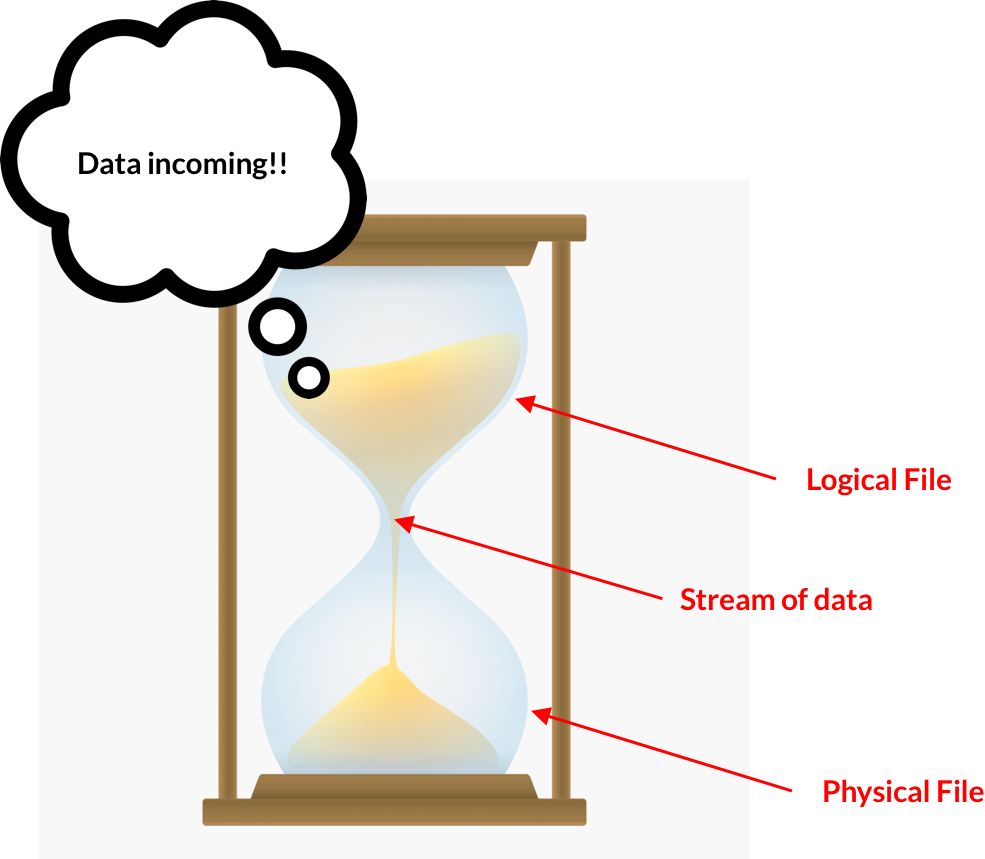
\includegraphics[width=0.8\linewidth]{images/week_8_notes_1_2.png}
            \end{center}
        \end{itemize}
    \end{itemize}

    \bigskip

    \underline{\textbf{Refernces:}}

    \bigskip

    \begin{enumerate}[1)]
        \item Tanebaum AS, Boss H. 2015. Modern Operating Systems. 4th Edition. New Jersy: Pearson Education, Inc.
        \item Kumar, S. (2010). \textit{File structures} [PowerPoint Slides]. Slide Share \href{https://www.slideshare.net/shyamujaco/file-structures}{link}
    \end{enumerate}
    % \item What is a Directory at the OS Level?
    % \item Operations on Directories
    % \item Example Directory Operations
    % \item Path Name Translation
    % \item Possible Directory Implementations
    % \item File Links
    \item Symbolic vs Hard Links

    \begin{center}
    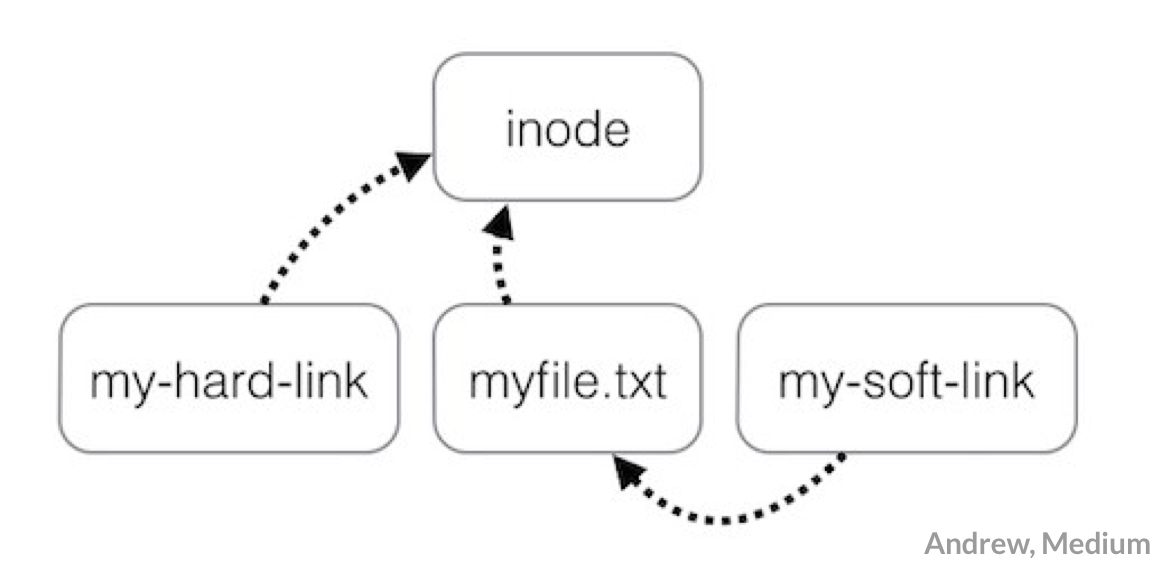
\includegraphics[width=0.8\linewidth]{images/week_8_notes_1_3.png}
    \end{center}

    \begin{itemize}
        \item \textbf{Inode}
        \begin{itemize}
            \item Is a database structure in a UNIX-style file system that describes
            a file system object such as a file or a directory $^{[1]}$
            \item Contains disk block location of the object's data $^{[1]}$
            \item Is a numerical equivalent of a full address $^{[2]}$
        \end{itemize}
        \item \textbf{Symbolic Link:}
        \begin{itemize}
            \item Is directory entry containing "true" path to the file
            \item Is a shortcut that reference to a file instead of inode value $^{[2]}$
        \end{itemize}
        \item \textbf{Hard Link:}
        \begin{itemize}
            \item Is a direct reference to a file via its inode $^{[2]}$
            \item Is second directory entry identical to first
        \end{itemize}
    \end{itemize}

    \begin{center}
    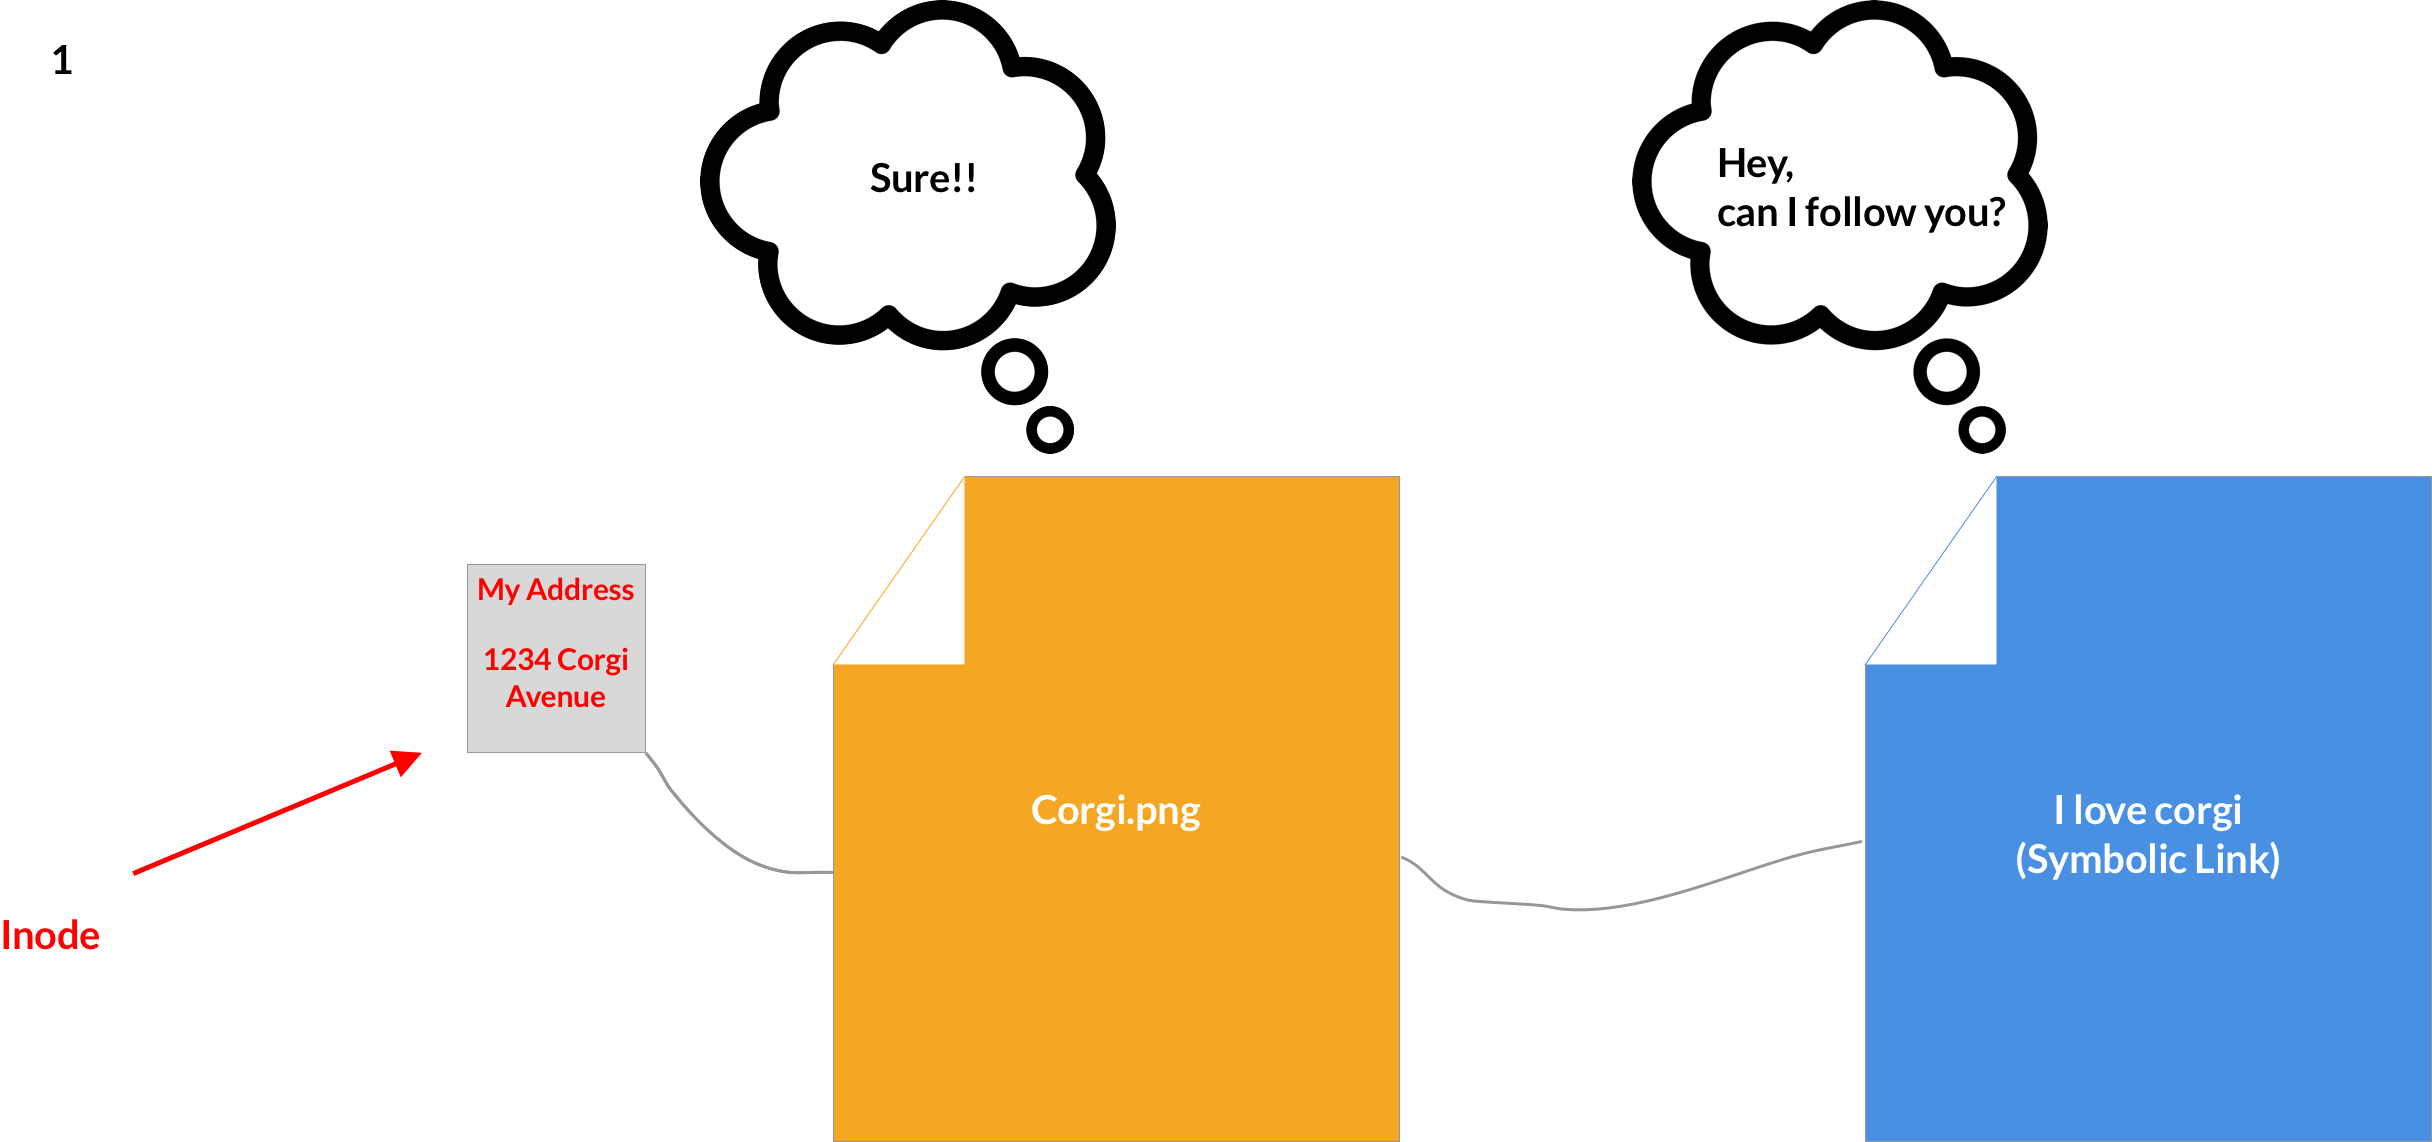
\includegraphics[width=0.8\linewidth]{images/week_8_notes_1_4.png}
    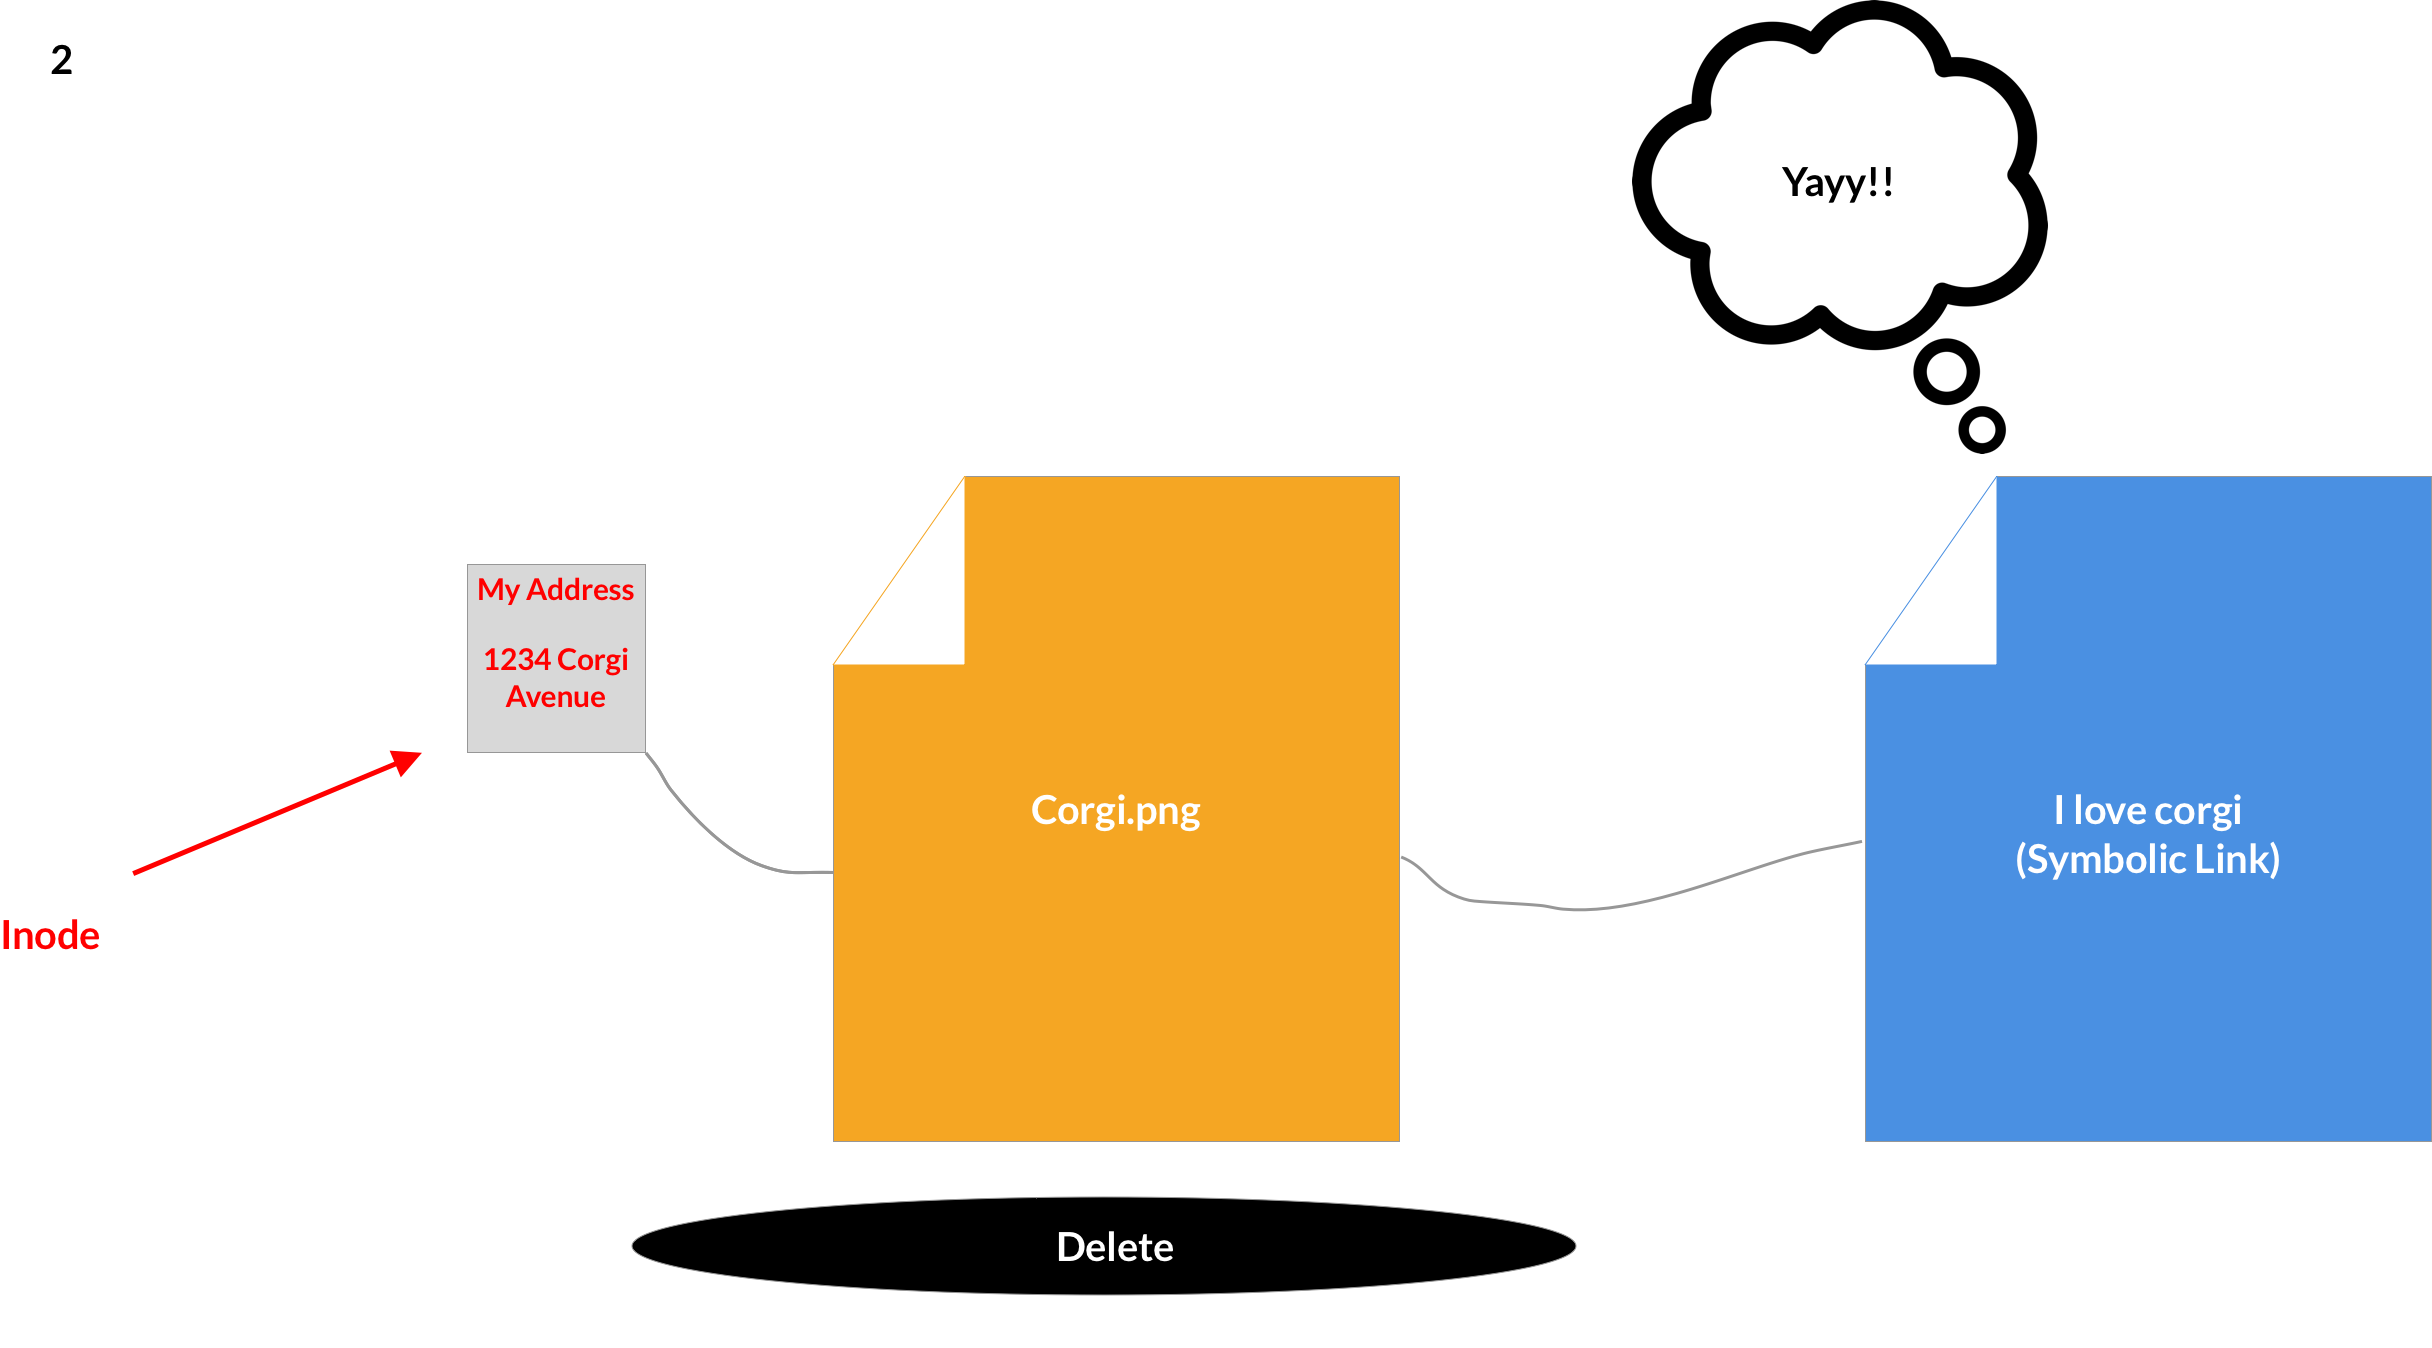
\includegraphics[width=0.8\linewidth]{images/week_8_notes_1_5.png}
    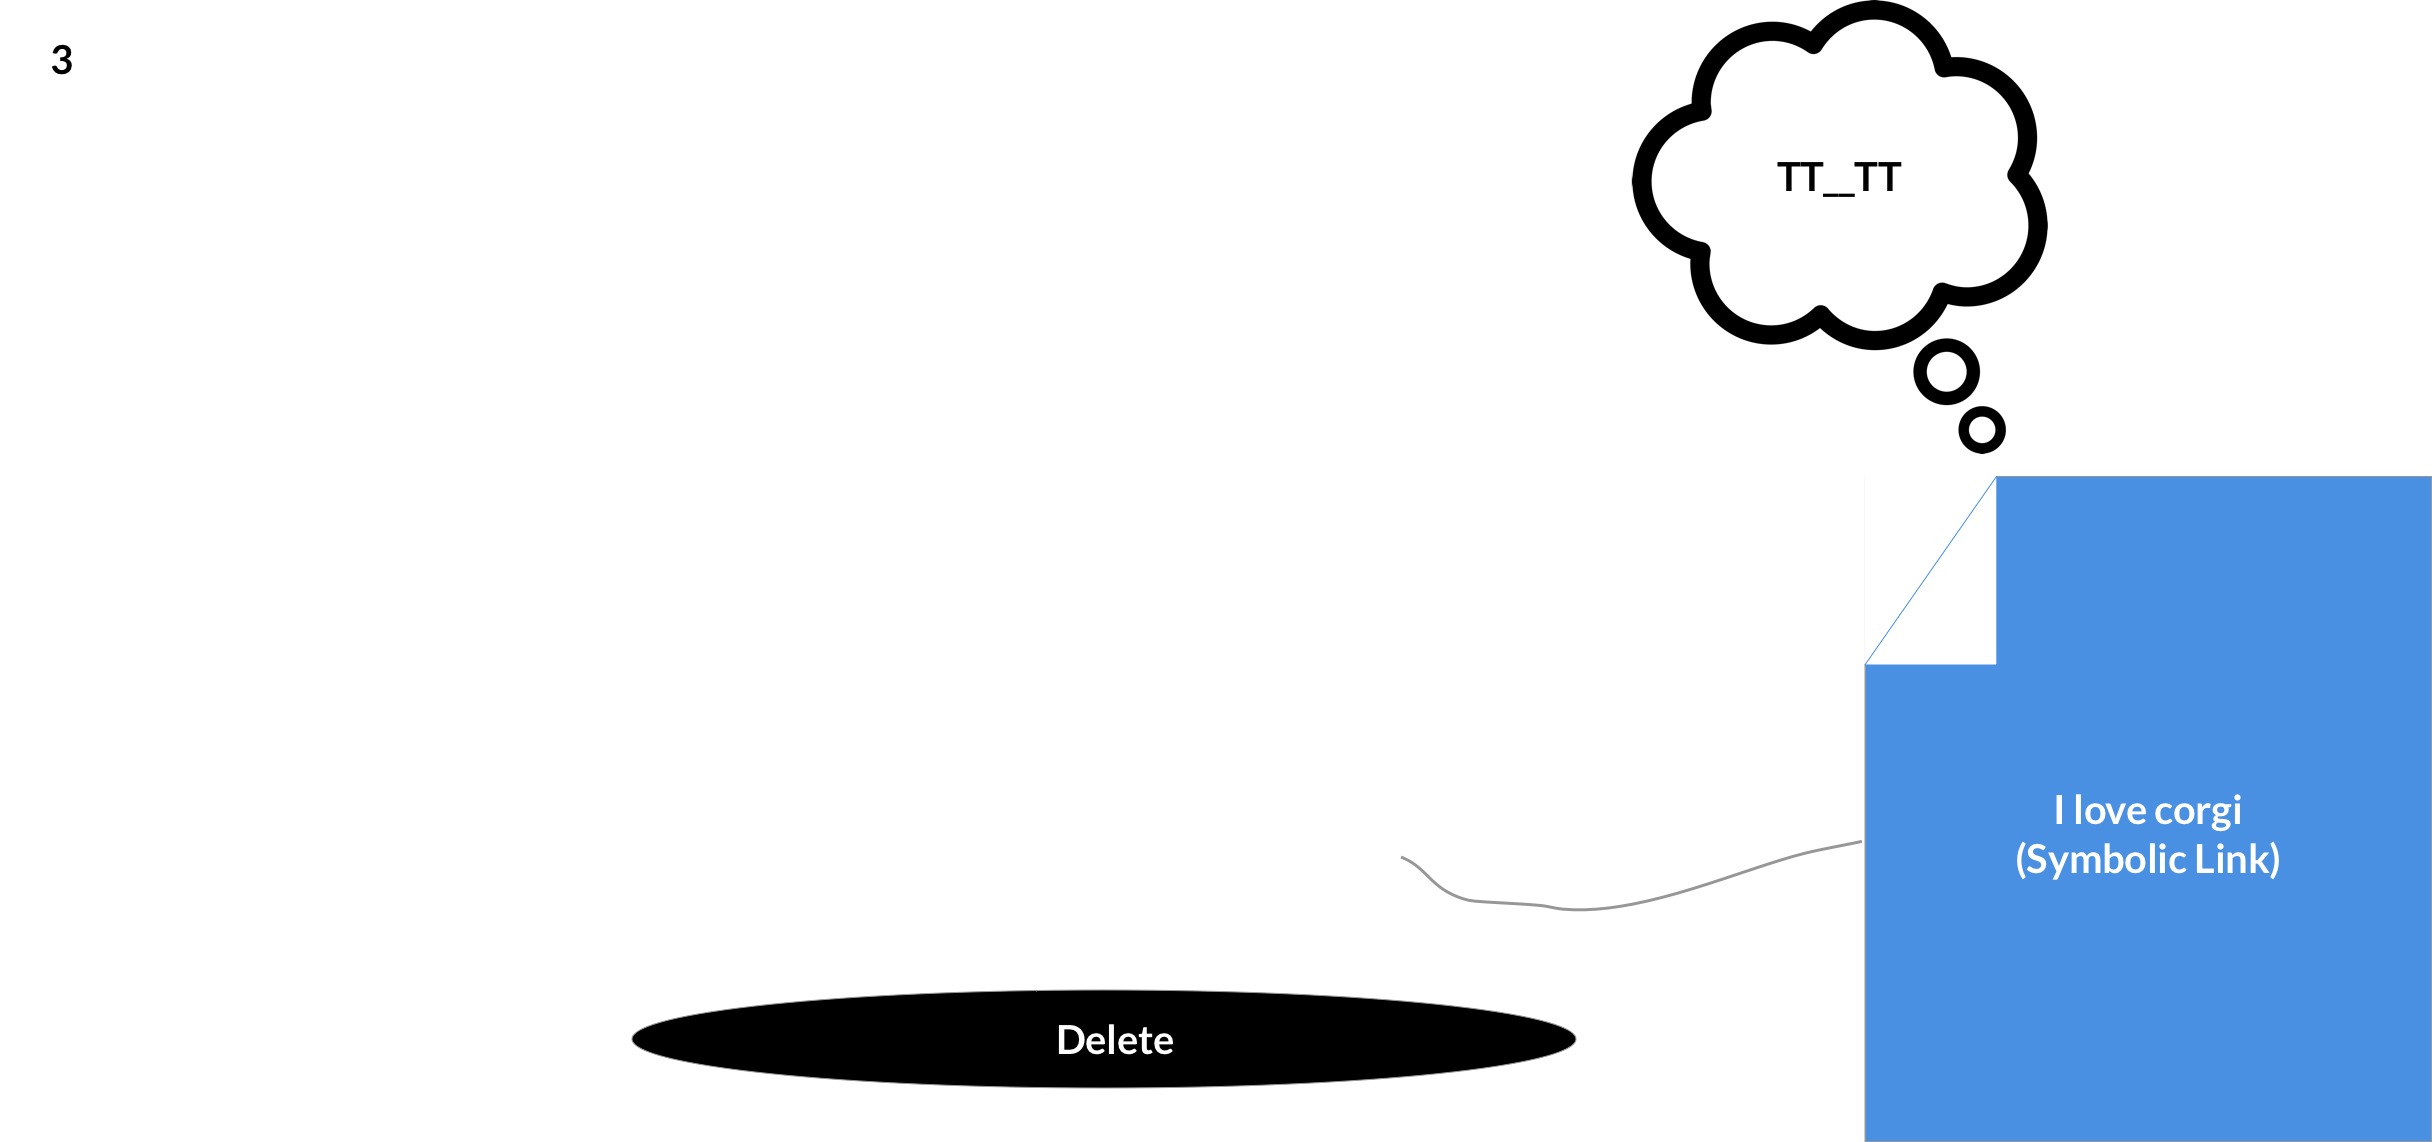
\includegraphics[width=0.8\linewidth]{images/week_8_notes_1_6.png}
    \end{center}

    \bigskip

    \underline{\textbf{Refernces:}}

    \bigskip

    \begin{enumerate}[1)]
        \item Wikipedia: inode, \href{https://en.wikipedia.org/wiki/Inode}{link}
        \item Andrew. (2018, January 16). \textit{Hard links and Symbolic links — A comparison}. Medium. \href{https://medium.com/@307/hard-links-and-symbolic-links-a-comparison-7f2b56864cdd}{link}
    \end{enumerate}
    % \item Issues with Acyclic Graphs
    % \item File Sharing
    \item Protection

    \begin{itemize}
        \item File systems implement some kind of protection system
        \begin{itemize}
            \item Who can access a file
            \item How they can access it
        \end{itemize}
        \item Protection system dictates whether given \color{green}\textbf{action}
        \color{black}\:by a given \color{orange}\textbf{subject}\color{black}\:on
        a given \color{red}\:\textbf{object}\color{black}\: should be allowed
        \begin{itemize}
            \item You can read and/or write your files, but others cannot
            \item You can read "etc/motd", but you cannot write it
        \end{itemize}
    \end{itemize}

    \begin{center}
    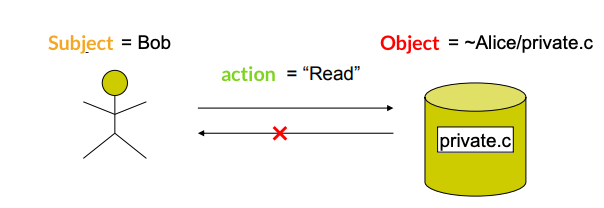
\includegraphics[width=0.8\linewidth]{images/week_8_notes_1_7.png}
    \end{center}
    % \item Types of Access
    % \item Representing Protection
    % \item ACLs and Capabilities
    % \item File System Implementation
    % \item Directory Implementation
    % \item Disk Layout Strategies
    % \item Contiguous Allocation
    % \item Linked Allocation
    % \item Indexed Allocation: Unix Inodes
    \item Unix Inodes and Path Search
    \begin{itemize}
        \item Unix Inodes
        \begin{itemize}
            \item Is what we see on typing `ls -li' command in terminal

            \begin{center}
            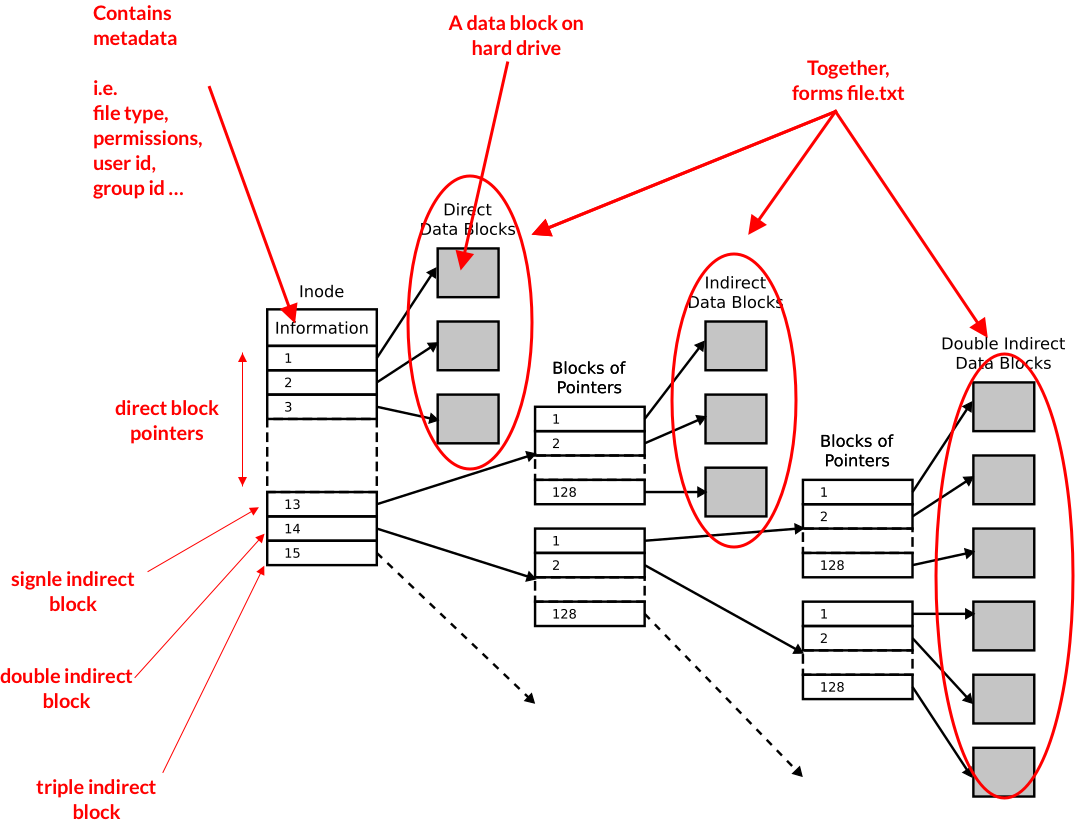
\includegraphics[width=\linewidth]{images/week_8_notes_1_8.png}
            \end{center}
            \item Describes where on the disk the blocks for a file are placed
            \item inode information is loaded to main memory $^{[1]}$
            \begin{itemize}
                \item Only for the corresponding files that are open
                \item NOT all are loaded
            \end{itemize}
        \end{itemize}
    \end{itemize}

    \bigskip

    \underline{\textbf{Refernces:}}

    \bigskip

    \begin{enumerate}[1)]
        \item Tanebaum AS, Boss H. 2015. Modern Operating Systems. 4th Edition. New Jersy: Pearson Education, Inc.
    \end{enumerate}
    \item File Buffer Cache
    \begin{itemize}
        \item Reads information from disk only once and then stores retrieved file blocks
        in memory until no longer needed $^{[1]}$
        \begin{itemize}
            \item Because reading from disk is slow
            \item Is common to read same part of disk multiple times

            \bigskip

            \underline{\textbf{Example:}}

            \bigskip

            \begin{enumerate}[1.]
                \item Reading email message, read the message for an edit, and
                read the message again when copying to folder
            \end{enumerate}
        \end{itemize}
    \end{itemize}

    \bigskip

    \underline{\textbf{Refernces:}}

    \bigskip

    \begin{enumerate}[1)]
        \item Linux System Administrators Guide: Chapter 6. Memory Management, \href{https://www.tldp.org/LDP/sag/html/buffer-cache.html}{link}
    \end{enumerate}
    % \item Caching Writes
    % \item Read Ahead
\end{itemize}

\end{document}